\documentclass{article}

% The LaTeX-to-CNXML translator makes use of Tralics, a LaTeX-to-XML conversion
% utility.  Tralics has implemented all the packages in the LaTeX base directory,
% and it also supports a good number of supplemental LaTeX packages.  These
% supplemental packages are included in the \usepackage{} statements below.
% Packages not in the LaTeX base directory or \usepackage{} statements in this
% template are not supported by Tralics and, hence, not supported by the
% LaTeX-to-CNXML converter.

% If you have a question as to whether a specific LaTeX command is supported,
% please refer to the "HTML Documentation of all TeX commands" section at
% http://www-sop.inria.fr/apics/tralics/.  Here you will find links to manual pages
% organized alphabetically by the first letter of the command.  These pages indicate
% how Tralics handles conversion of each supported command, which informs how the
% LaTeX-to-CNXML translator behaves.

% To prepare your LaTeX document for import, copy the body of that document from its
% source and paste it into this template between the \begin{document} and \end{document}
% statements.  Do not attempt to use any packages other than the ones contained in this
% template.  You may, however, insert user-defined macros directly in this template
% before the \begin{document} statement.  Following this preparation, check to see if
% your template-compliant document can generate a .dvi (.pdf) using latex (pdflatex).
% If so, then your document is ready for import; if not, you must modify your document
% to generate an output file using only the packages supported by Tralics as described
% above.

%Is this in base?
%\usepackage{epsfig}
%\usepackage{epstopdf}

% Tralics supports the following AMS packages
% (see http://www-sop.inria.fr/apics/tralics/packages.html for details on full/partial
% support of package commands)
\usepackage{amsbsy,amscd,amsfonts,amsgen,amsmath,amsopn,amssymb,amstext,amsthm,amsxtra}

% Tralics supports \includegraphics and \scalebox, but not all other graphicx package
% commands; check the web documentation on supported commands before attempting to use
% other commands in the graphicx package:
\usepackage{graphicx}

% We must specifically invoke the verbatim package as follows to direct Tralics to handle
% the verbatim environment properly:
\usepackage{verbatim}

% Tralics also allows the following packages:
% (see http://www-sop.inria.fr/apics/tralics/packages.html for details on full/partial
% support of package commands)

%\usepackage{alltt}
%\usepackage{array}
%\usepackage{bracket}
%\usepackage{calc}
%\usepackage{delarray}
%\usepackage{eucal}
%\usepackage{eufrak}
%\usepackage{fancyverb}
%\usepackage{fix-cm}
%\usepackage{fixltx2e}
%\usepackage{flafter}
%\usepackage{fontenc}
%\usepackage{fp}
%\usepackage{graphpap}
%\usepackage{html}
%\usepackage{ifthen}
%\usepackage{index}
\usepackage[utf8]{inputenc}
%\usepackage{latexsym}
%\usepackage{lipsum}
%\usepackage{makeidx}
%\usepackage{minimal}
%\usepackage{mml}
%\usepackage{natbib}
%\usepackage{newlfont}
%\usepackage{oldlfont}
%\usepackage{shortvrb}
%\usepackage{showidx}
%\usepackage{soul}
%\usepackage{syntonly}
%\usepackage{textcase}
%\usepackage{textcomp}
%\usepackage{tloop}
%\usepackage{theorem}
%\usepackage{upref}

%-------------------------------------------------------------------
% You can insert user-defined macros (using the supported packages
% only) here...
\DeclareUnicodeCharacter{03B2}{\beta}
%-------------------------------------------------------------------

\begin{document}

\section{Objectives}
After completing this section you should understand the Booth's Multiplication Algorithm for the multiplication of signed binary numbers.
Booth's Multiplication Algorithm provides an efficient and relatively simple algorithm for using machine-register operations for the multiplication of two's complement binary values.

%I'm considering merging this with the above.
\section{Preparation}
This sections assumes familiarity with with binary addition at the machine level and with the two's complement representations of negative numbers.
%Possibly make recommendations here

\section{Introduction}
The process of binary multiplication is significantly more computationally complex than that of addition.
Multiplication is often defined recusivly as repeated additions.
%Consider providing full definition
Using this approach to calculate $11 \times 23$, you would start with 0 and add 11 to it 23 times.
This method is terribly inefficient, and execution time varies wildly depending on the values multiplied.
%There are alot of superlatives here
For example, the equivalent problem of calculating $23 \times 11$, requires 12 fewer operations).
Since as computer architects we dislike unpredictability, we must make several modifications to this algorithm before it resembles something that could be done well in hardware.
%There is not background to this statement of Architects and efficiency.

%This section seems math-y, maybe should be re-arranged in the article
\section{Shift-and-Add Multiplication}
The ``shift-and-add'' method for binary multiplication is the binary-equivalent of multiplication by partial products.
To review, this method involves multiplying one number, hereafter called the multiplicand, or $M$, by successively more significant digits of the other number, hereafter referred to as the multiplier, or $Q$.
The results of these individual multiplications are referred to as ``partial products'', and the sum of these partial products is the final product.

Another way to think of this is as follows: let $Q$ be an n-digit binary number and let the $i^{th}$ bit of $Q$ be denoted $q_i$ (this text goes by the convention that the $0^{th}$ bit of a binary value is the rightmost or least-significant bit).
Then the significance (or ``place-value'' as you learned it in elementary school) of $q_i$ is $2^i$.
We can then express the problem $M \times Q$ as $M \times (q_{n-1} \times 2^{n-1} + q_{n-2} \times 2^{n-2} + \ldots + q_{0} \times 2^{0})$.
Each one of the products $(q_i \times 2^{i}) \times M$ is a partial product.
For binary values, there are only two values a partial product may be: if $q_i = 0$, then the result is simply $0$; otherwise the result is $M \times 2^i$.

Consider the following calculation of the multiplication of 001011 and 010111, which, in two's complement notation, is 11 and 23, respectively.
Since many architectures use fixed-sized registers to hold data, we will use the same number of bits to represent both $M$ and $Q$.
%diagram goes here
\pagebreak
\begin{figure}
\centering
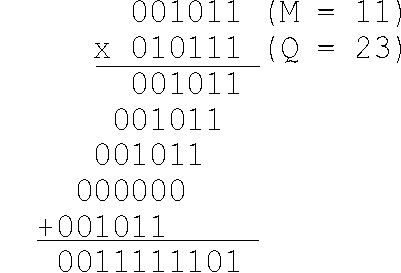
\includegraphics[scale=0.7]{saam3.pdf}
\caption{Shift-and-Add Multiplication}
\end{figure}

We see already a vast improvement in the performance of this algorithm, compared to the repeated additions method.
Each partial product shown corresponds to an addition operation (+M or +0).
In every line except the first, there is also an implicit shift operation, corresponding to the significance of the bit being multiplied with $M$.
Again, recall that the significance of bit $q_i$ is $2^i$, so if $q_i = 1$, then the partial product looks like $M$ followed by $i$ trailing 0s.
Much like multiplying by powers of $10$ in decimal, we are simply ``shifting'' the bits in M to more significant place values.

Compare the method described above, which involves the addition of 5 partial products and 4 shifts for this problem, to the method proposed in the introduction, which requires 23 additions.
Even though this is only one example, it should give you a good idea of how much better the performance of this algorithm is.
The speedup is even greater if one considers that, on some machines, shift operations can potentially take less time than addition operations.

\pagebreak

\section{Problems with the Shift-and-Add Method}
There are several issues that prevent us from directly implementing the shift-and-add algorithm into hardware.
To begin with, most ALUs are only capable of adding two numbers together at a time.
This means a \emph{running product} must be calculated for every partial product, instead of calculating the final product at the very end of the process.
The running product is initialized to 0, and for every partial product calculated the new running product is the sum of the old running product plus the partial product.
We will call the space used to store the running product register A.
Since we are begining our discussion of computer design problems, we will similarly refer to the space used to store the multiplicand and multiplier as register M and register Q, respectively.

Notice also that as the algorithm progresses, the position at which the numbers are added incrementally slides to the left.
It is a much simpler task to design a machine that always adds into the same location and then shifts the running product to the right by 1.
We will refer to this operation as a \emph{sign-preserving right shift}, or \emph{sprs} for short.
This is also known as an \emph{arithmetic right shift}.

Finally, we need to consider register size.
In the previous example, the numbers we multiplied were represented as 6-digit binary values; their result, however, required 10 bits to represent.
In general, if two n-bit numbers are multiplied, then the result can require as many as 2n bits to represent.
Thus, the convention is to store the result of multiplication between two registers.

\pagebreak

\begin{figure}
\centering
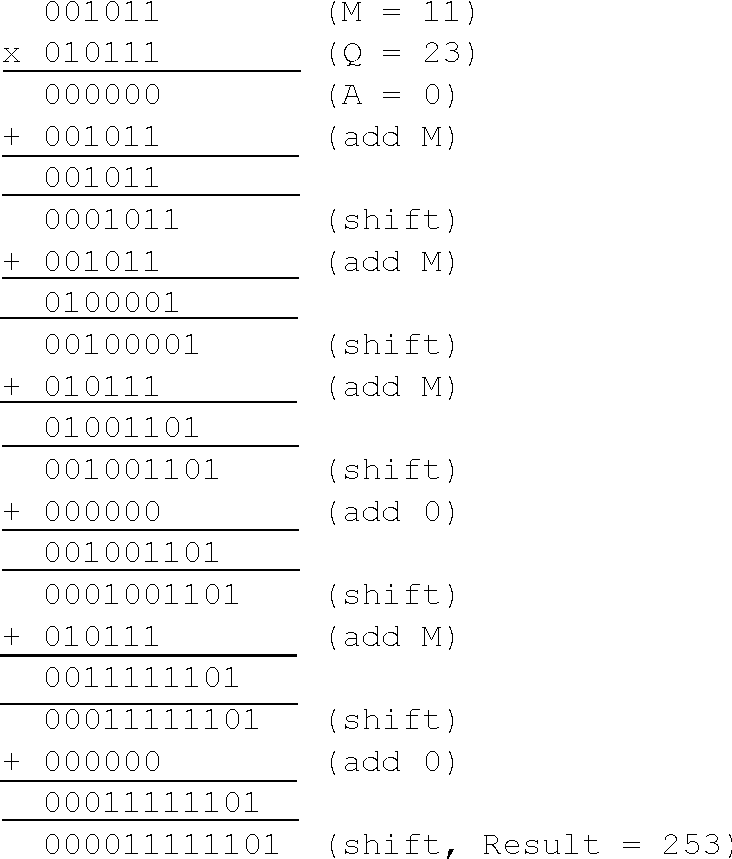
\includegraphics[scale=0.7]{isaam2.pdf}
\caption{Improved Shift-and-Add Multiplication}
\end{figure}

\section{Improved Shift-and-Add Multiplication}
Figure 2 shows an improved version of the shift-and-add multiplication algorithm.
You should study it so that you understand how the problems which were discussed in the previous section are addressed in this new shift and add method.

There is still another computer design issue which could make this method easier to implement in hardware: in the last example, the bit in register Q we are using to calculate a partial product is always positioned one to the left of the previous bit we used, or else it is the right-most (least significant, \emph{lsb}) bit of register Q when the multiplication starts.
We could instead choose to always examine the \emph{lsb} of register Q, and for every right shift operation on register A, we would also do a right shift on register Q.
Thus, when the algorithm finishes, all of the previous values in Q will have been discarded.
This will allow us to be even more efficient: instead of using another register to store the lower half of the product, we can use register Q, because, for every bit discarded from Q, we can place into Q's most significant bit (\emph{msb}) the \emph{lsb} of A, saving ourselves from using a whole other register!

\pagebreak
\begin{figure}
\centering
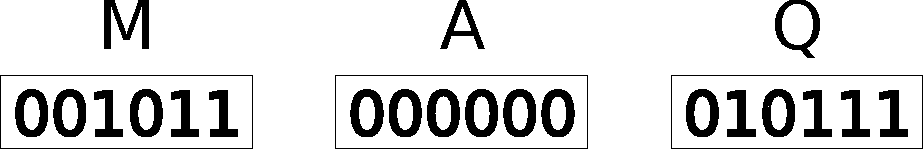
\includegraphics{init.pdf}
\caption{Registers M, A, and Q, initialized for the multiplication of 11 and 23}
\end{figure}

\section{The Problem with Negative Numbers}
Consider the multiplication of the following 4-bit 2's complement numbers: 0011 (3) and 1011 (-5).
We expect a result of -15 (11110001); however, currently the method we have been developing is unable to distinguish between signed and unsigned values, and would multiply 3 by 11 (the unsigned decimal value of 1011).
One way around this behavior would be to calculate the absolute values of our multiplier and multiplicand.
Then, after the positive product was calculated, if either the multiplicand or the multiplier are negative (but not both), calculate the two's complement of the product.
This is a suboptimal solution from a design point of view, as it introduces the need for extra hardware and/or processing of binary numbers whenever we wish to multiply.

\section{Booth's Encoding}
In 1951, Andrew Booth introduced an alternative method for multiplying two's complement numbers.
At its heart is the observation that a number like 0111, which is understood to mean $2^2 + 2^1 + 2^0 = 4 + 2 + 1 = 7$, can also be thought of as $2^3 - 2^0 = 8 - 1 = 7$.
This can be written (encoded) as $100\bar{1}$, where 1 and 0 have their understood meanings, and $\bar{1}$ represents represents $-1$.

    In general, it can be shown that any number of the form $2^n + 2^{n-1} + ...
+ 2^{n-k}$ is equal to $2^{n+1} - 2^{n-k}$.
When the number is composed of multiple sequences like these, such as $2^7 + 2^6 + 2^5 + 2^1 + 2^0$ or 011100011, apply the rule to each valid sub sequence, which in this case would be $2^8 - 2^5 + 2^2 - 2^0$ or $100\bar{1}0010\bar{1}$.
For use in binary multiplication, this method translates into the following: for every sequence of 1s in the multiplier (Q), replace the rightmost (least significant) 1 with $\bar{1}$, replace the first 0 on the left of the sequence (if it exists) with 1, and set all the 1s between the positions of the bits you just modified to 0 (if there is no leading 0, simply flip all the other bits of the selected sequence to 0).
For the case where the ``sequence'' of ones is a single bit, ie $...010...$,
the appropriate encoding would be $...1\bar{1}0...$,
which is correct because $2^n = 2^{n+1} - 2^n$.
%TODO better math

This method also works if the multiplier is negative.
There are three cases: either the most significant bit is not followed by anything (that is, it is both the least- and most-significant bit), or it is followed by 0 (such as 1001, or -7), or else it is followed by 1 (such as 1101 or 1111, which are -3 and -1 respectively).
In the first case, we convert the single bit to $\bar{1}$, which is correct since `1' actually represents $-1$ as a 1-bit number in two's complement notation, 

In the second case, the most significant bit is converted to $\bar{1}$, representing a subtraction.
Since this bit represents a value larger than any value which can be represented in the bits to the right of it, the final value will be negative.

In the third case, consider the largest leftmost sequence of 1s in Q (this is, in fact, the sequence which indicates the binary value is negative).
By Booth's method, the rightmost bit in this sequence will be converted into $\bar{1}$, since it is either followed by a 0 or else not followed by anything (if it were followed by a 1, then the sequence we selected would not be the \emph{largest} leftmost sequence of 1s).
Then, all the bits to the left of the selected bit will converted to 0s.
Again, this guarantees that the most significant non-zero bit in the multiplier (Q) is negative, so that the whole number itself will be negative.

So far we have only shown that our encoding process will preserve the sign of the original value.
To show that the two values are equivalent, first recall that the value of $N$, a negative binary number in two's complement representation, can be expressed as:
\[-2^k + \sum_{i=0}^{k-1} (n_i \times 2^i)\]
where $n_i$ is value of the $i$th bit of $N$, and $k$ is the \emph{position} (not value) of the rightmost bit in the largest leftmost sequence of 1s in $N$.
Similarly, the encoded value of $N$, which we will call $N^{\prime}$, can be expressed as:
\[-2^{k^{\prime}} + \sum_{i=0}^{k^{\prime}-1} (n_i^{\prime} \times 2^i)\]
where $n_i^{\prime}$ is the value of the $i$th bit of $N^{\prime}$ and $k^{\prime}$ is the position for the most significant bit with value $\bar{1}$.
From our discussion of case three, we know the position of the rightmost bit in the largest leftmost sequence of 1s in $N$ is the same as the position of the most significant bit with value $\bar{1}$ in $N^{\prime}$, so we know that $k$ and $k^{\prime}$ are equal.
Finally, since the sums represent positive values (if they do not, we have picked the wrong values for $k$ and $k^{\prime}$), and since from our earlier discussion in this section we have shown (informally) why Booth's algorithm works for positive values, we can now say the two equations are equivalent.
(Note: be careful not to think the two equations say the same thing: the values of $n_i^{\prime}$ can be 0, 1, or -1 ($\bar{1}$), whereas the values of $n_i$ can only be 0 or 1)

\section{Booth's Algorithm in Hardware}
    At the hardware level we are only allowed the use of 0 and 1 to represent values, so we instead examine pairs of bits.
Scanning a binary number from right to left, the pair `10' signifies the beginning of a sequence of 1s and thus corresponds to a subtraction (or $\bar{1}$).
The pair `01' signifies the end of a sequence of 1s and corresponds to an addition.
The pairs '00' and '11' signify that no arithmetic operations need occur (the equivalent of adding 0).
Since we would like to stay as close as possible to the algorithm outlined earlier, all cases will still require a shift.

    In order to examine pairs of bits, we add an extra 1 bit register, called $\beta$ (or Beta) to hold the bit shifted out of Q.
$\beta$ is initialized to 0, so that at the start of the algorithm, if the least significant bit of Q is 1, it will read a pair `10' and execute a subtraction.
Keep in mind now that whenever a shift occurs, the least significant bit of A is moved into the most significant bit of Q, and the least significant bit of Q is moved into $\beta$.
The old value of $\beta$ is discarded.

\begin{figure}[h]
\centering
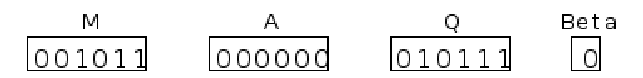
\includegraphics{init2.pdf}
\caption{Registers M, A, Q, and Beta, initialized for the multiplication of 11 and 23}
\end{figure}

\section{Visualizing Booth's Multiplication}
Everything we have considered so far for an appropriate machine level algorithm to multiply two's complement values has been implemented as a JHAVÉ visualization.
Instead of using the form of the previous examples, it more closely resembles the way the algorithm might be executed in hardware, placing explicitly the multiplicand and multiplier in registers M and Q respectively, and storing the final result in registers A and Q.
An example run-through is provided below, as well as a link to a use-case video.
Step through the visualization as many times as you need, answering the questions as they appear, then proceed on to the exercises.

%\section{Example Run of the Visualization}
%After starting the JHAVÉ client and selecting ``Booth's Multiplication Algorithm'', an input generator window will appear with four text fields, two for decimal input and two four binary input, and a menu to select register size.
%You may choose your own values for the visualization, or use the default values provided (if you are having trouble getting the input generator to take your values, make sure you selected an appropriate register size for your values).
%When you are ready to begin the visualization, press ``OK''.

%\begin{figure}[h]
%\centering
%\includegraphics{vis1.pdf}
%\end{figure}

%The next few snapshots of the visualization 

%-------------------------------------------------------------------
% to create references, un-comment \bibliographystyle{plain} and
% un-comment \bibliography{myBIBfile} and re-name its arguemnt(s)
% to point at the .bib file(s) containing the BibTeX references:

%\bibliographystyle{plain}
%\bibliography{myBIBfile}

\end{document}
